%!TEX root=report.tex
\new
\section{Experimental evaluation}
\label{experiments}

Having proposed and argued for the semantic gossip mechanisms, we addressed the first research question defined in Section \ref{sec:intro}.   Now, we turn our attention to the 
sencond and third research questions.  To address those we build a prototype of our ideas and conduct a series of experiments.

%we want to evaluate their effectiveness. % We aim at a better performing consensus protocol with the same resilience.  
%We conduct experiments to give answer to the sencond and third research questions defined in Section \ref{sec:intro}.
%following main questions:
%\begin{itemize}
%\item is there a gain in performance of consensus, and how much, using each of the mechanisms, and combined, in relation to none ?
%\item is the vulnerability of consensus increased in the presence of increasing number of dishonest nodes ?
%\item \fd{is that all?}
%\end{itemize}

\subsection{Methodology}
\label{ref:method}

Gossip networks are typically built having nodes connecting to a number of randomly chosen peers.
A basic concern is how different topologies 
could affect gossip and the proposed mechanisms and thus impact the consensus protocol using gossip.   To address this concern, our study starts with a characterization of possible topologies obtained from a gossip arrangement of nodes, and their properties, in Section \ref{sec:topos}.
%
We then present system configurations and deployments to conduct experiments in Section \ref{sec:setup}.
%Using a class of representative topologies with the system configurations described we conduct experiments aiming to answer the above mentioned questions.
%\fd{review}
The first set of experiments aims to answer the second research question, being
reported in Sections \ref{sec:overall} to \ref{sec:latency-cdfs}. 
We used increasing workload 
aiming to assess the relation of throughput and latency.
The workload is increased by stepwise enabling Tendermint to handle more 
instances concurrently.
%\fd{review}
Regarding the third research question, resilience evaluation is reported Section \ref{sec:resilience}.  
We fixed a workload and assessed resiliency by 
stepwise increasing the number of byzantine nodes in the network from 0\% to 30\%, 5 by 5\%.   For each case, we observe again the result of throughput and latency.
In Section \ref{sec:msgLoss} we evaluate throughput and latency under increasing message loss rate.

%Finally, we additionally report on the observed impact of signatures validation needed in the semantic layer, in Section \ref{sec:signatureImpact}.
%\fd{DO WE ?}















\subsection{Choice and Distributed Generation or Network Overlays}
\label{sec:topos}

Due to the random generation of network overlays by the gossip protocol, 
we have to ensure that the overlays used in the experiments are representative, not leading to distortion in the measures obtained.
Moreover, we have to provide a distributed algorithm to generate these overlays. In this section we discuss how the overlays used in the experiments can be obtained and their characteristics.

\subsubsection{Network overlay definition}

A network overlay is a graph $G(V,E)$, where $V$ represents the set of
processes running the experiment (validator nodes) and $E: V \times V$ represents the set of bi-directional network connections between processes.  $G$ is simple (a process does not connect to itself and there is only one edge among any two nodes) and non-directed
(an edge means communication in both directions is possible).  The following definitions are useful in next sections:
\begin{itemize}
	\item $peers_G(p \in V) := \{q \in V : (p, q) \in E\}$ is the set of processes directly
	connected to $p$ in the overlay $G$.
    \item $degree_G(p \in V) := |peers_G(p)|$ is the number of connections process $p$ has in
  the network overlay $G$.
   \item   $outPeers_G(p \in V)$ and $inPeers_G(p)$: the set of outbound and inbound peers of $p$, i.e., 
	processes $q \in peers_G(p)$ to which $p$ is expected to respectively dial
     and establish a connection, or accept a connection request.
\end{itemize}

\paragraph{Soundness} A network overlay is valid, said sound, if the following requirements are fulfilled:
\begin{itemize}
\item connected: $G$ is connected, i.e., there is a path
built out of edges in $E$ among any two processes in $G$.
\item minimum neighbourhood: for fault-tolerance,  each node in 
the overlay is required to have
at least $f+1$ neighbours, where $f$ is the allowed number of faulty processes,
ensuring that any node is always connected to at least one honest node.
In our case $f < n/3$, $n$ being the total number of nodes.
\end{itemize}

% For any two processes $\{p, q\} \in V$, if $(p, q) \in E$ then there is a 
% connection between processes $p$ and $q$ in the network overlay $G$.
%In order to properly model the behavior of the network, a network overlay $G$
% has the following properties:   
% \begin{itemize}
% 	\item $G$ is a simple graph, i.e., $(p, q) \in E \implies q \neq p$, as processes
%   do not connect to themselves;
%     \item  $G$ is a undirected graph, i.e., $(p, q) \in E \implies (q, p) \in E$,
%   as connections are bi-directional.
% \end{itemize}
%

%On a more specific terms, it is interesting if the process $p$ is able to
%classify its peers in two categories:
% UNNEDED:  Also, $outPeers_G(p) \cup inPeers_G(p) = peers_G(p)$ and 
% $outPeers_G(p) \cap inPeers_G(p) = \emptyset$.
% The classification of peers in outbound or inbound peers is antisymmetric:
% $\forall p,q \in V$ if $q \in outPeers_G(p)$ then $p \in inPeers_G(q)$.
% In practical terms, this means that process $p$ will dial process $q$,
%while $q$ will not dial process $p$, but wait for a connection request from it.
%## Random overlays

%Since there is a large amount of possible network overlays for a given 
%set of processes, we produce and analyze randomly generated network overlays.

\subsubsection{Distributed generation}
\label{sec:distributedGeneration}

Given a network overlay $G$ to be used in an experiment (or instantiation of
the protocol), each process $p \in V$ should be able to compute the 
set $peers_G(p)$ with which they should be connected in the adopted network overlay.
Each process $p$ has to be able to identify its $in$ and $outPeers_G(p)$.
%
%\subsubsection{Network overlay characterization}
For its generation, we characterize a random network overlay using three parameters:
\begin{itemize}
	\item  $n$: the number of processes in the network, i.e., $n = |V|$.
    \item  $k$: the connectivity parameter, which can be seen as the target value for
  $degree_G(p)$ for every $v \in V$.
    \item $s$: the seed employed to randomly select the connections between processes
  in the network overlay.
\end{itemize}

Notice that $n$ and $k$ are parameters for the generation of a class of random
network overlays, while $s$ allows to uniquely identify each individual random
network overlay belonging to that class.   
%
Using the same seed and random number generator, a deterministic distributed algorithm can be used to compute the same network at each distributed process. In a distributed algorithm, if each of the $n$ nodes chooses $x$ neighbours to connect, the expected final number of neighbours of a node\footnote{$E_{nbr} = A + B - C$ where: $A$ is the number of neighbours chosen by this node, $A=x$; $B$ is the number of nodes that choose this one has neighbour, as $n$ nodes choose this one with probability $x/n$, $B=n \times x/n$; and $C$ is the number of mutual choices that may take place, as two nodes choose to be neighbours with probability $(x/n)^2$, we have that for $n$ nodes $C = (x/n)^2 \times n$.   With this, $E_{nbr} = x + n \times x/n - (x/n)^2 \times n = 2 x - x^2/n$}
is $E_{nbr} = 2 x - x^2/n$.
%resulting graph $G$ will have average $degree_G$
%
%For example, in a network with $n=128$, since $f \leq n/3$ and $k\geq f+1$ each node should have at least $k=43$ neighbours. If each node independently chooses $k$ neighbours, the expected average $degree_G$ of nodes is $E_{nbr}=71.5$.
%To minimize the extra redundancy of the resulting overlays,
%we refine the simple approach above such that each node chooses
%$k'$ other nodes, and
To generate networks in which $E_{nbr}$ approaches the desired connectivity $k$, %where nodes have in average $k$ neighbours.
%each node has with $E_{nbr}$ approximating $k$.
%i.e. $k = n \pm \sqrt{n^2-n k'}$. Thus,
in the distributed algorithm we use $x$ obtained from the above relation. 
%, where 
%%%%%%  >>  $x =\lceil n - \sqrt{n^2-n k} \rceil$.
%we used $k' = n \pm \sqrt{n^2-n k}$.  As for $1 \leq k \leq n$, $(n + \sqrt{n^2-n k}) \geq n$,
%we take $k' = n - \sqrt{n^2-n k}$. % resulting in $0< k'\leq n$.
For instance, in a network with $n=128$, if we want nodes to have in average $k = 43$ neighbours, $x$ should be $23,69$. So we use $x = 24$: each node chooses randomly $24$ neighbours. 

Our deterministic algorithm for distributed overlay generation has the following main parts: assuming input $\langle k, n, seed \rangle$ and using the same random generator: (a) from $k,n$ find $x$ as above; (b) in the same order of nodes in $n$, for each node randomly choose $x$ neighbours; (c) if the network is not connected or there exists any node with less than $k=f+1$ neighbours, repeat from (b), otherwise adopt the network.  
To ease the process of finding a network with the needed minimum connectivity we can slightly increase $x$.

\paragraph{Classification}

\begin{figure}[htbp]
	\centering
	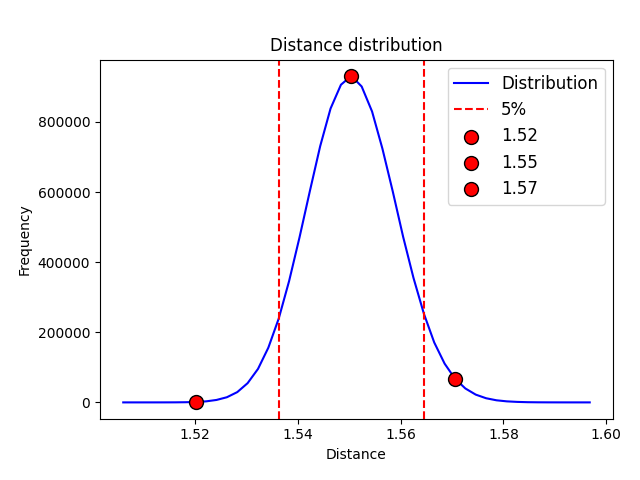
\includegraphics[%width=\columnwidth,
  height=5cm]{figures/n32-topology-distance-distribution.png}
	\caption{Distance distribution of the random generated overlays for n=32,k=13.8.}
	\label{fig:topologyDistribution}
\end{figure}

\begin{figure}[htbp]
	\centering  
	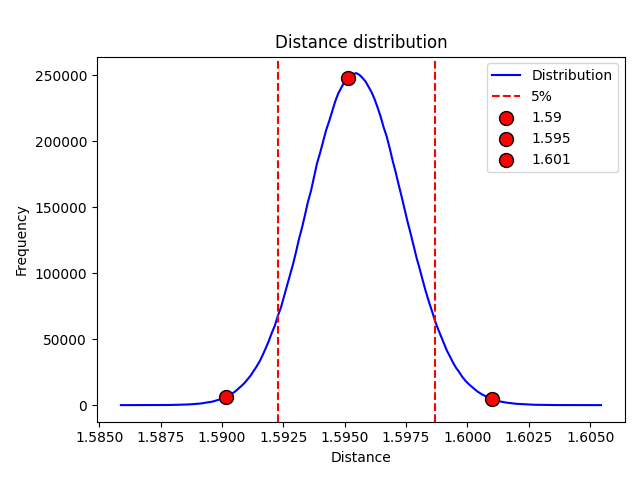
\includegraphics[%width=\columnwidth, 
     height=5cm]{figures/n128-topology-distance-distribution.png}
	\caption{Distance distribution of the random generated overlays for n=128,k=51.3 }
	\label{fig:topologyDistribution128}
\end{figure}

Once we have a distributed generation algorithm, we have to evaluate if radom generated topologies are free from any bias that may impact the results.
Since the distance among nodes is a fundamental aspect of gossip performance,  we classify overlays using their average shortest path length among any pair of nodes.  We call this metric the distance of an overlay and in Figures \ref{fig:topologyDistribution} and
\ref{fig:topologyDistribution128}
we present the distance distribution for overlays with $n=32$, $x=8$ leading to $k=13.87$; and $n=128$, $x=29$ leading to $k =51.43$.
%With this, we generate a population of sound overlays and, for each one we compute its distance, associating the triple $\langle k, n, seed \rangle$ to the value obtained.   After this,
We select sound instances from this population that are in different extremes of the distance distribution (below 5\% and above 95\%), as well as samples in the center of the distribution.  Experiments are run with each selected overlay instance, showing in Figures \ref{fig:n32TopologyComparison} and  \ref{fig:n128TopologyComparison} that they have comparable impact on all semantic gossip techniques, meaning that the techniques are not favored by the choice of different   topologies generated with the same arguments.  %\fd{TO DO:  In each fig we have to choose if we show the upper or lower part.   And then reshape it to become readable (font size in axes, legends, ...). The lower part shows more directly that the semantic gossip mechanisms are not impacted by different topologies in the distance distribution - for same conectivity parameter.}
%
Once this is observed, we follow the studies with the average distance topology (center of distribution).

%Each selected instance is used to configure a set of Tendermint validator nodes, these validators compute the same topology with the refined algorithm above, build the network connections, run the same workload, and extract performance metrics.  
%Experiments show that 
%showing equivalent results. Which leads to conclude that that the random generation of sound overlay networks with same parameters $\langle k, n \rangle$ lends networks with equivalent performance.

%\begin{figure*}[htbp]
%	\centering
%	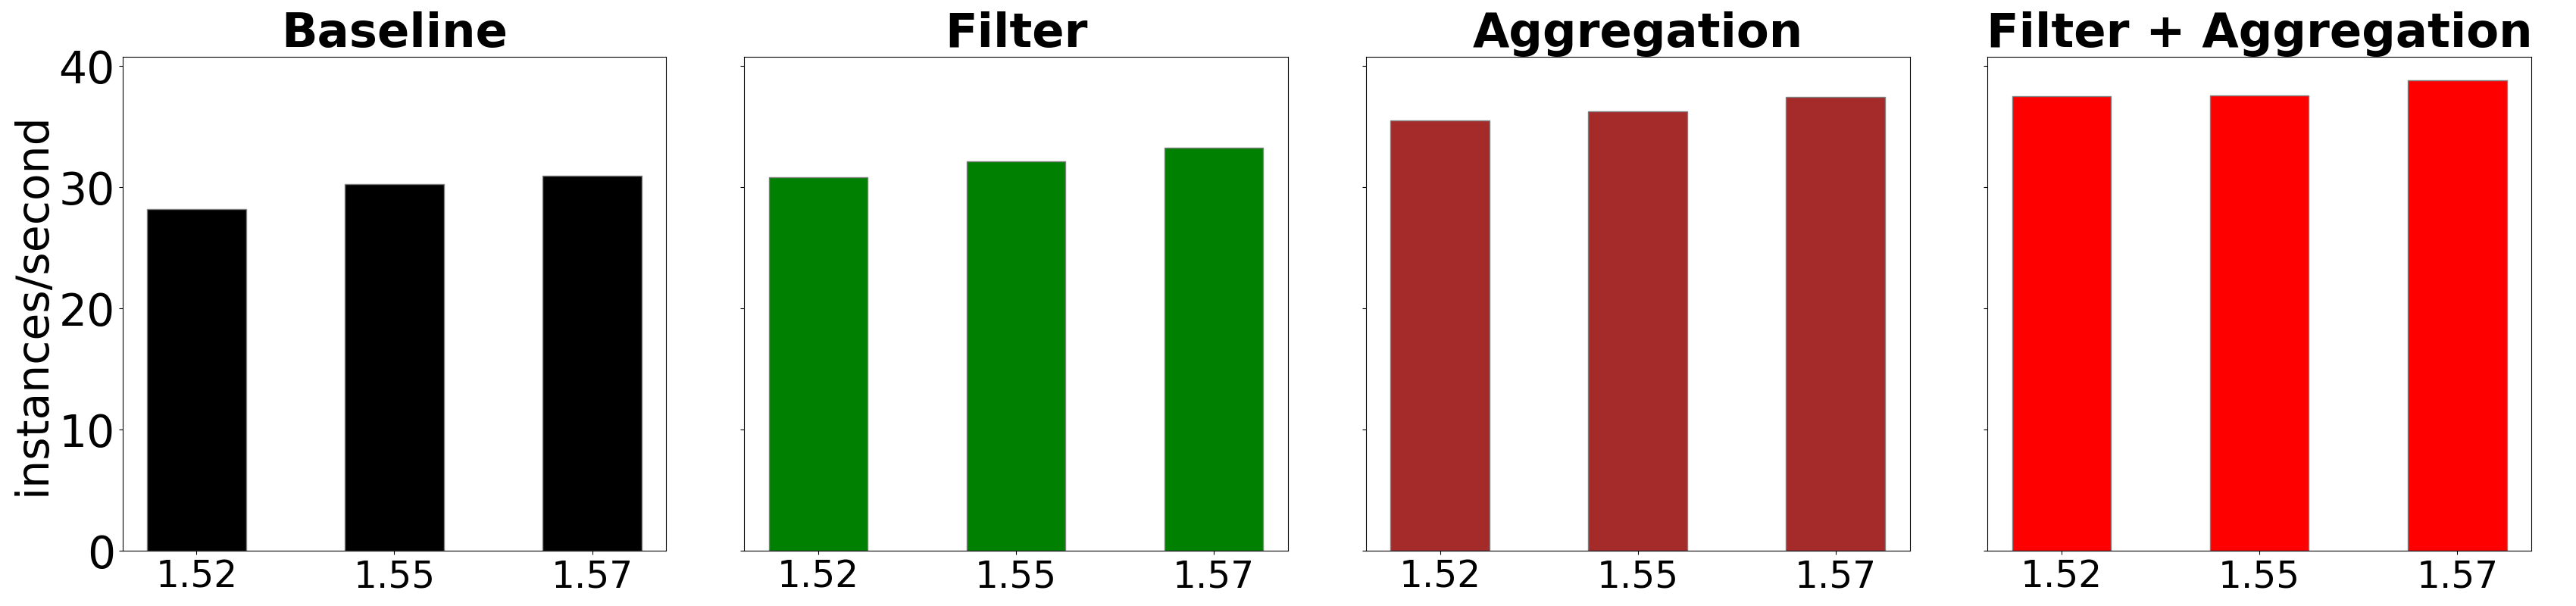
\includegraphics[
 %      height=3.5cm]{figures/topo-thr-hist-32n.png}
%	\caption{Throughput of the best throughput/latency relation points, for different setups and different average node distances (x axis for each setup) in a network with n=32 and k=13,8.}
%	\label{fig:n32TopologyThrComparison}
%\end{figure*}


\begin{figure*}[htbp]
	\centering

	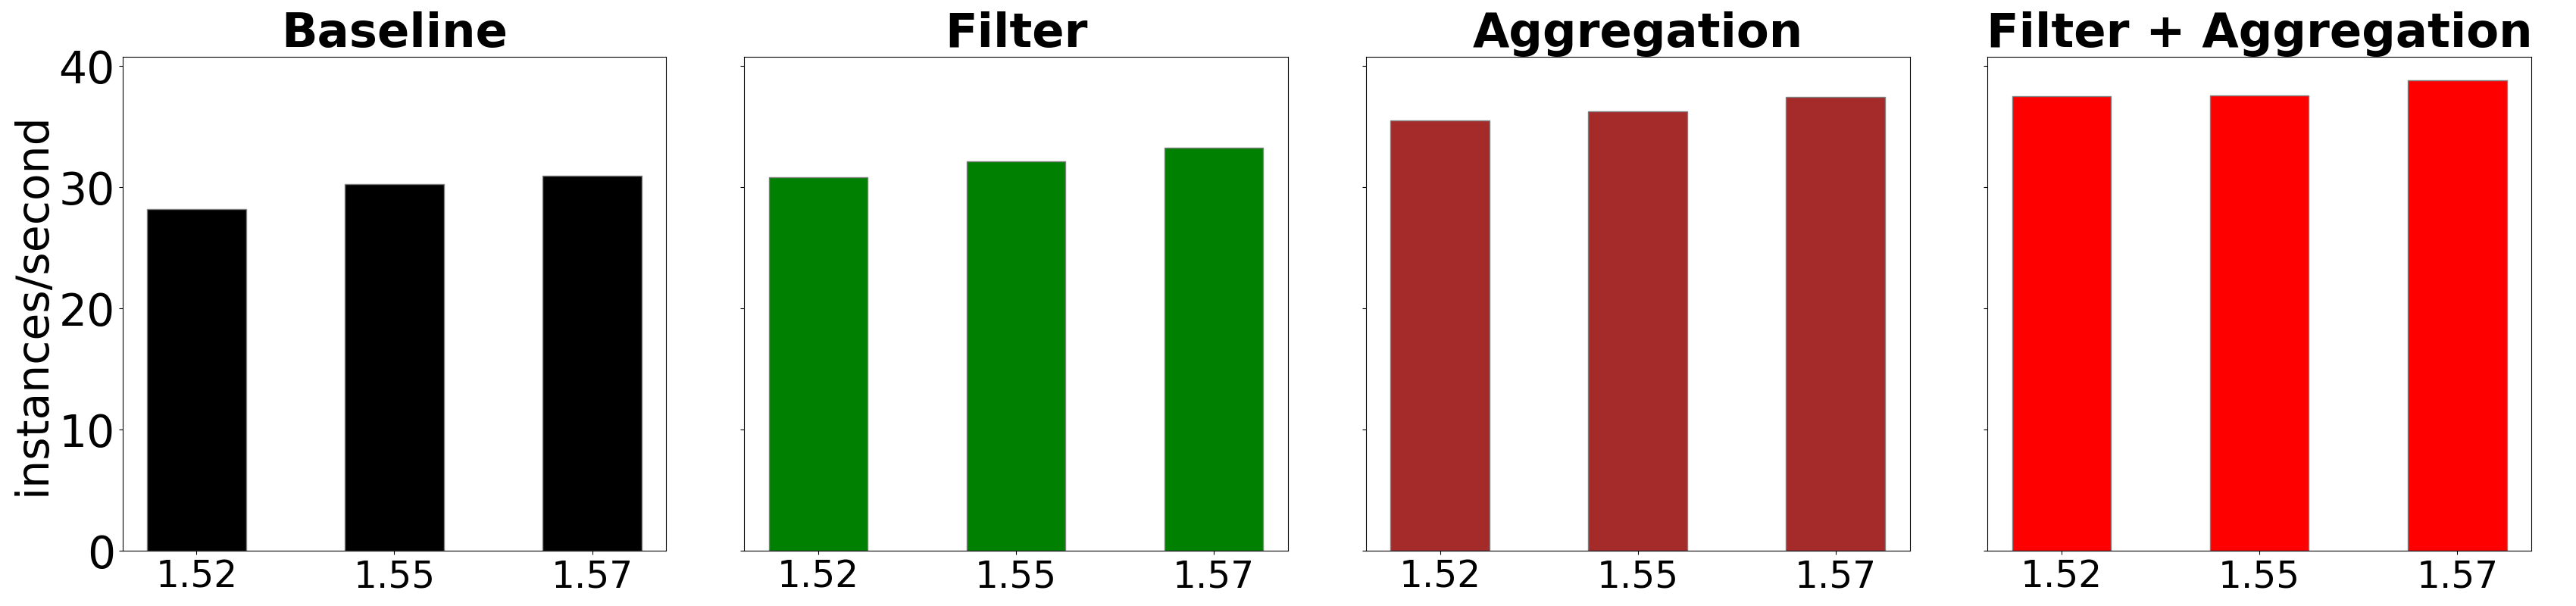
\includegraphics[
       height=3.5cm]{figures/topo-thr-hist-32n.png}

\vspace{5mm}

	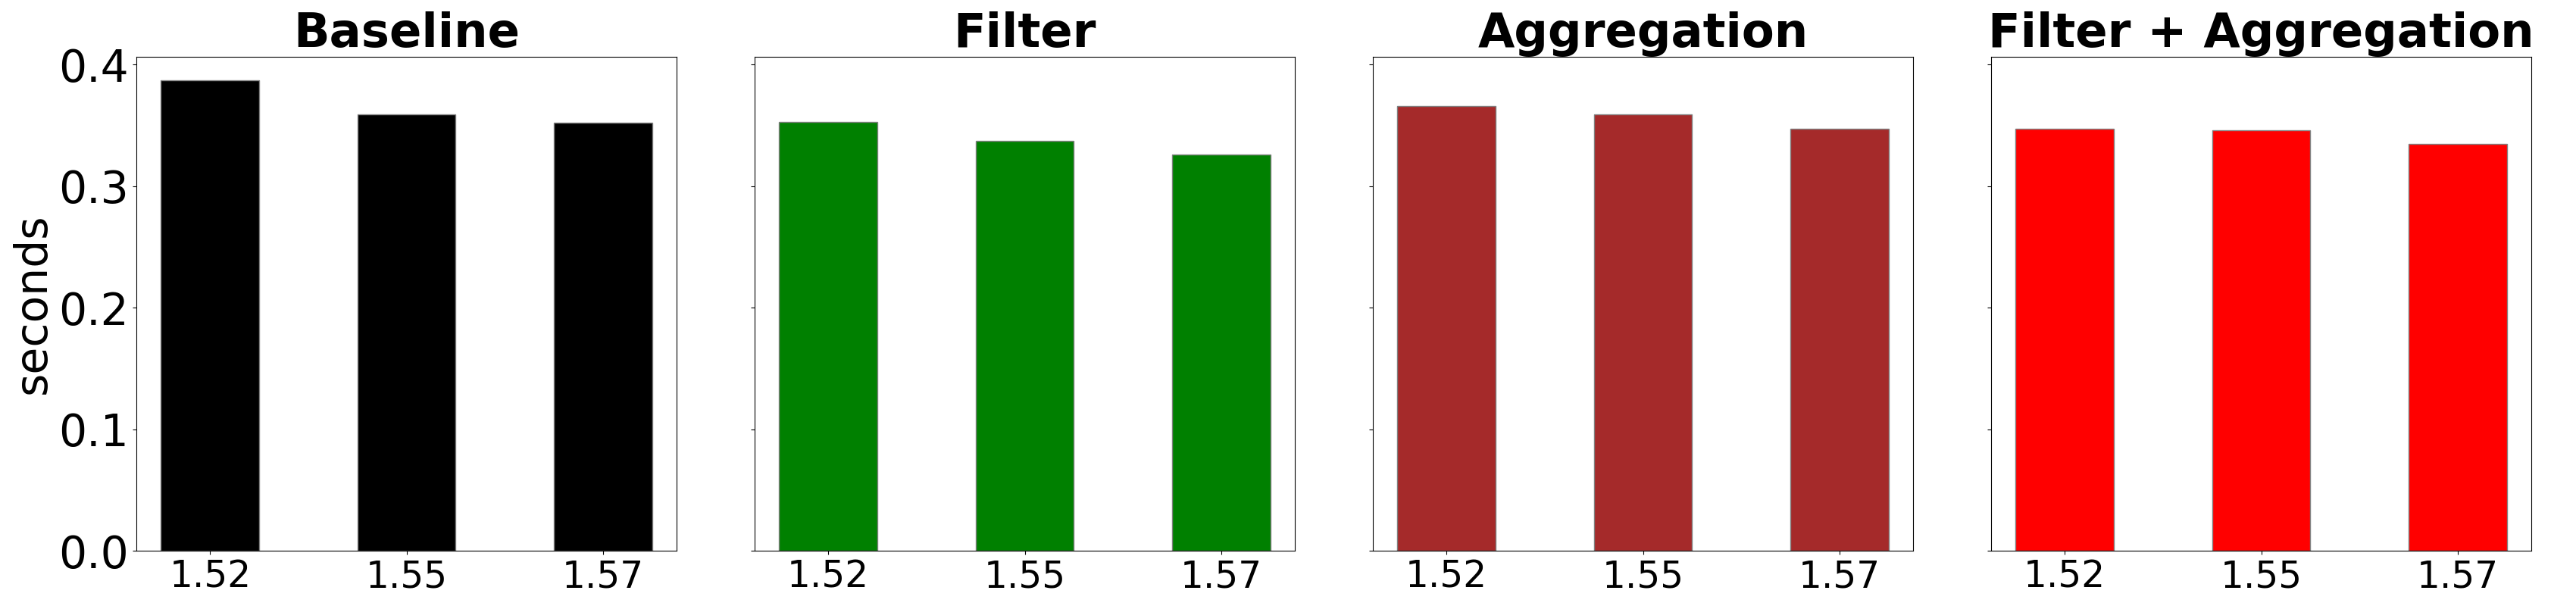
\includegraphics[height=3.5cm]{figures/topo-lat-hist-32n.png}
	\caption{Throughput (above) and latency (below) of the best throughput/latency relation points, for different setups and different average node distances (x axis for each setup) in a network with n=32 and k=13,8.}
	\label{fig:n32TopologyComparison}
\end{figure*}

\begin{figure*}[htbp]
	\centering
	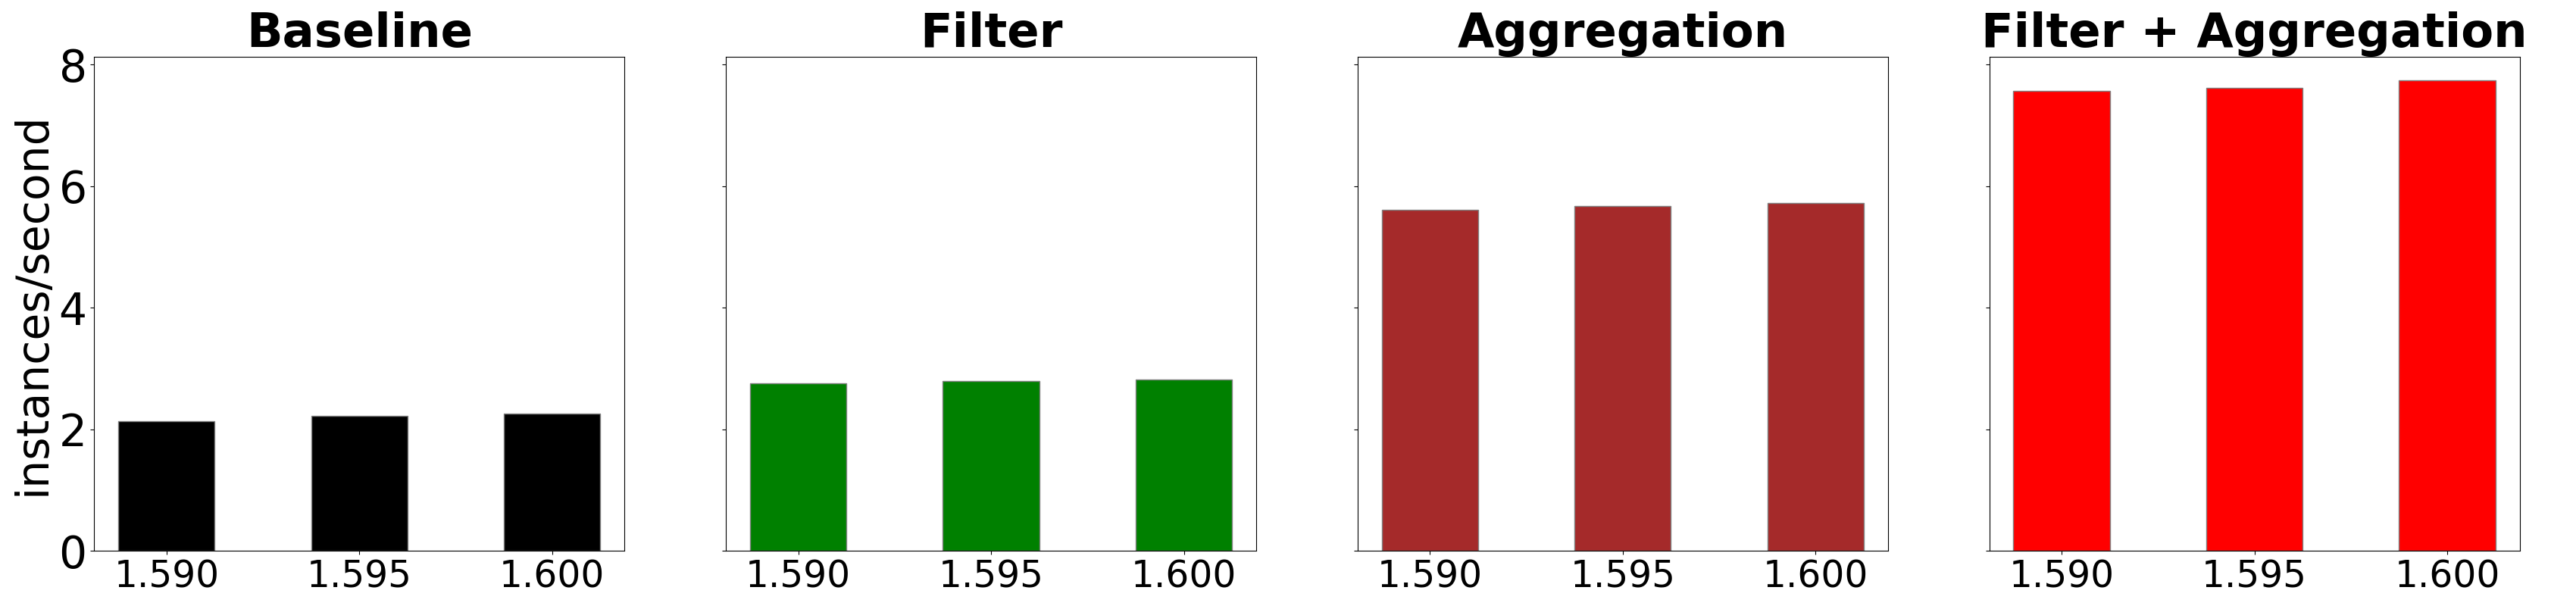
\includegraphics[height=3.5cm]{figures/topo-thr-hist-128n.png}
\vspace{5mm}

 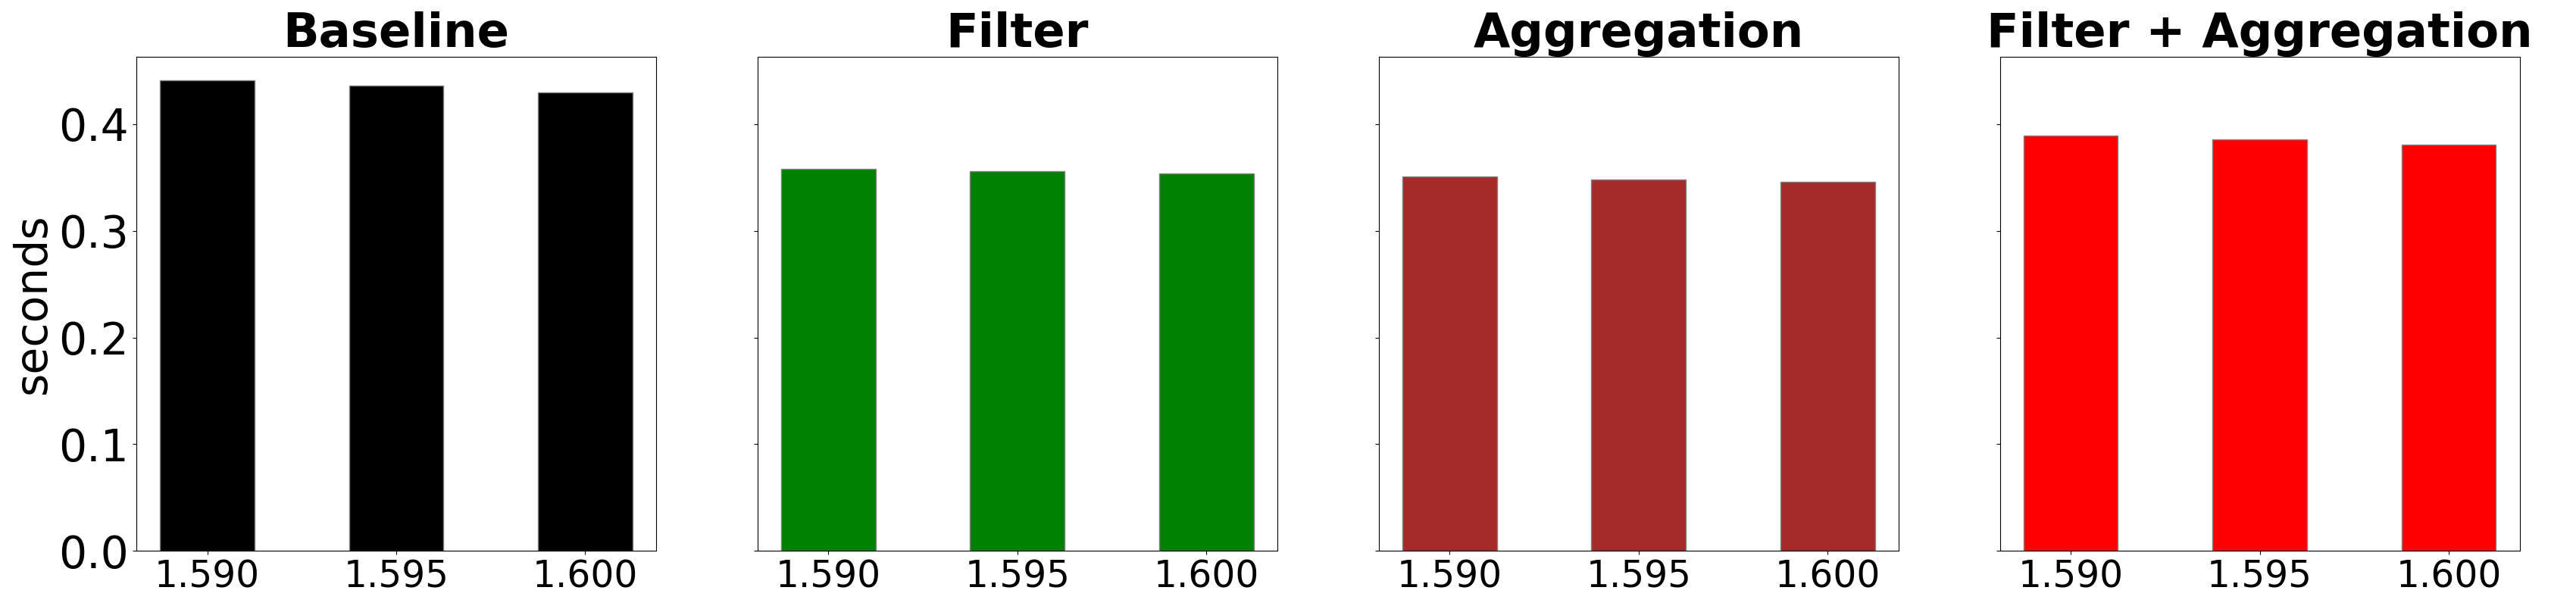
\includegraphics[height=3.5cm]{figures/topo-lat-hist-128n.png}
 
	\caption{
 Throughput (above) and latency (below) of the best throughput/latency relation points, for different setups and different average node distances (x axis for each setup) in a network with n=128 and k=51,43.}
	\label{fig:n128TopologyComparison}
\end{figure*}




% \begin{table}[h!]
% 	\begin{tabular}{c c c c c }
% 		\hline
%     Topology  &        &       &       & Filtering+  \\ 
% 	 mean & Baseline   & Filtering    & Aggregation    & Aggregation  \\  \hline

% 	1.590  		& 		...		&		&		&   \\
% 	1.595  		& 				&		&		&   \\
% 	1.600  		& 				&		&		&   \\ \hline \\
% 	\end{tabular}
% 	\caption{Saturation point throughput for different topologies, using none (Baseline), Filtering,
% 	Aggregation and Filtering and Aggregation semantic gossip mechanisms with Tendermint.}
% \end{table}


%\subsubsection{Randomness of the method -- \fd{REMOVE?}}

%Randomness is related to the overlay generation method, and not the overlay itself.  An overlay generation method is said fair if each possible edge is included in a resulting overlay with same probability. 

%An edge $(p,q)$ is included when process $p$ chooses $q$ as neighbour or vice-versa. If the assumption of proper random choice is valid, the probability of a process $p$ choosing another one $q$ as neighbour is the same for any process $q$, thus the probability that edges are included in an overlay is the same for different edges.


% The generation of the random overlay considers the set $V$ of processes, where $|V| = n$.
% The randomness is introduced by producing random permutations of the set $V$.
% This means to turning the set $V$ to an ordered set (a sequence), where the
% position of each element $v \in V$ in the ordered set is randomly chosen:

% 1. Each process $v \in V$ computes a random permutation of the set $V$ of
%    processes: `rnd_perm(v, s, V)`.
% 1. Each process $v \in V$ selects the first $k$ other processes from the
%    produced random permutation, namely `selected(v, s, k, V)` = \{ the $k$
%    first processes $p \in$ `rnd_perm(v, s, V)` with $p \neq v$ \}.

% The random network overlay is produced from the computed `selected(v, s, k, V)`
% sets, so that:

% 1. The outbound peers of process $v$ are defined by the set `selected(v, s, k, V)`.
% 1. The inbound peers of process $v$ are all processes $p \in V$ that have
%    randomly selected $v$.
%    More formally, is the set `selected_by(v, s, k, V)` =
%    \{ $p \in V$ so that $p \in$ `selected(p, s, k, V)` \}.
% 1. The set of peers of a process $v$ is: $peers_G(v)$ =
%    `selected(v, s, k, V)` $\cup$ `selected_by(v, s, k, V)`.

% Note that the same process $p$ can be on both `selected(v, s, k, V)`, thus $p$ is
% a process to which $v$ will dial, and `selected_by(v, s, k, V)`, meaning that
% $v$ should expect process $p$ to dial it.
% However, since $peers_G(v)$ is the union of the two sets, the above defined
% process $p$ should count only once as peer of $v$.
% In practical terms, this means that $v$ should keep only one of the two
% connections possibly established with process $p$.

% ## Analysis

% The source of randomness of this method is the production of the ordered sets
% `rnd_perm(v, s, V)`.
% We assume that they are actually random, so that for any two diferent processes
% $v, p \in V$, `rnd_perm(v, s, V)` and `rnd_perm(p, s, V)` are two uncorrelated
% permutations of set $V$.
% The same should apply for different random seeds `s` and `s'`, which should
% produce uncorrelated  `rnd_perm(v, s, V)` and `rnd_perm(v, s', V)`.

% If the assumption of proper random choice is valid, the probabily of $p \in$
% `selected(v, s, k, V)` should be the same for any proces $p \in V, p \neq v$.
% The probability in this case is $k/(n-1)$, as the combination of $k$ random
% selections (independent and uniform) of values from the set $V - \{v\}$, which
% contains $n-1$ elements.

% The same rationale applies for the composition of `selected_by(v, s, k, V)`.
% The probability that the process $v \in$ `selected(p, s, k, V)` is $k/(n-1)$, for
% any other process $p \in V$.
% Assuming that the production of those sets is completely independent, the
% expected number of other processes $p$ that have selected $v$ is given by the
% probability of being on each of those sets ($k/(n-1)$) times the number of
% sets considered ($n-1$).
% Thus, the expected size of set `selected_by(v, s, k, V)` is $k$, that is,
% the same size of set `selected(v, s, k, V)`.

% In term of the total number of peers, the method ensures that we have
% $|peers_G(v)| \geq k$.
% This is garanteed as |`selected(v, s, k, V)`| = k.
% To this minimal size we should add the size of set `selected_by(v, s, k, V)`,
% which expected value is $k$ as well, but removing the members from the
% intersection of both sets.
% This means that $|peers_G(v)|$ = $k$ + |`selected_by(v, s, k, V)`| -
% |`selected(v, s, k, V)` $\cap$ `selected_by(v, s, k, V)`|.

% The expectation for the number of peers $peers_G(v)$ of a process $v$ in the
% random overlay $G$ is then $2k$ minus expected size of the above mentioned
% intersection.
% To derive a more precise expectation, we would need to derive the expected size
% of the intersection `selected(v, s, k, V)` $\cap$ `selected_by(v, s, k, V)`.


\subsection{System configuration and deployment}
\label{sec:setup}

We implemented Tendermint, the gossip communication layer, and the Semantic Gossip extensions in Go.
We rely on libp2p~\cite{libp2p} to establish and maintain communication
channels between pairs of processes.
Libp2p channels are build atop TCP connections, and provide encryption,
multiplexing, flow control, and network-level batching.
Although libp2p channels are reliable, our implementation may discard messages when queues connecting different routines are full, as a way to prevent slow
processes from blocking the main transport routine.
In addition, libp2p connections may be dropped when receivers are much slower
than senders; although the dropped connections are reestablished, some messages may be lost. Temporary disconnections between peers, however, do not compromise the network connectivity.

The same Tendermint implementation is used to build different setups. In the first, \emph{Baseline}, Gossip is used. The other setups use Semantic Gossip, being \emph{Filtering} only, \emph{Aggregation} only, and 
\emph{Filtering and Aggregation} combined.
Either using Gossip or Semantic Gossip, each process opens a libp2p channel to a random subset of processes as discussed in section \ref{sec:distributedGeneration}.

The above setups are experienced with networks of 32 and a 128 nodes.
%
Load is generated at each node, upon its turn to propose a 
block for validation. I.e. whenever a node is enabled to propose a block, it does.
%
To experience higher workloads, we implemented a varying window of concurrent consensus instances allowed.
This means that while a block proposed by a node is being validated, further 
block(s) can be proposed by the next nodes.
The number of blocks that may be under validation concurrently, in the network, 
is called window.   The population of messages in intermediate nodes increases with the window sizes, allowing to better understand the effect of the mechanisms proposed.

A single instance of the experiment is characterized as a combination of: 
a given a topology (triple $\langle k, n, seed \rangle$);
one of the four setups; 
a concurrency window size; 
the time-span and the size of proposed value. 
For each combination of topology and setup, we start with window 1 and 
increment until saturation.  For each window size, 
we let the nodes free to propose and decide values as fast as possible, during a times-pan of 4 minutes.
%\fd{We use 1024 bytes as size of proposals.  ?}
%
Each node has a module where the load is generated and instances decided are 
delivered.
This allows to build an output log with all the deliveries and their consensus latencies.
%with the consensus latency for the values they generated. 
Also, during the experiment, a node periodically records working variables such as the size of the gossip queues presented with Figure \ref{fig:architecture_sg}, number of filtered messages and number of aggregated messages.


As deployment environment we use CloudLab's\cite{Duplyakin+:ATC19} bare metal machines. 
We use machines type M400 from CloudLab's Utah cluster with configuration eight 64-bit ARMv8 (Atlas/A57) cores at 2.4 GHz (APM X-GENE) and 64GB ECC Memory (8x 8 GB DDR3-1600 SO-DIMMs).


\subsection{Overall performance}
\label{sec:overall}

\begin{figure}[htbp]
	\centering
	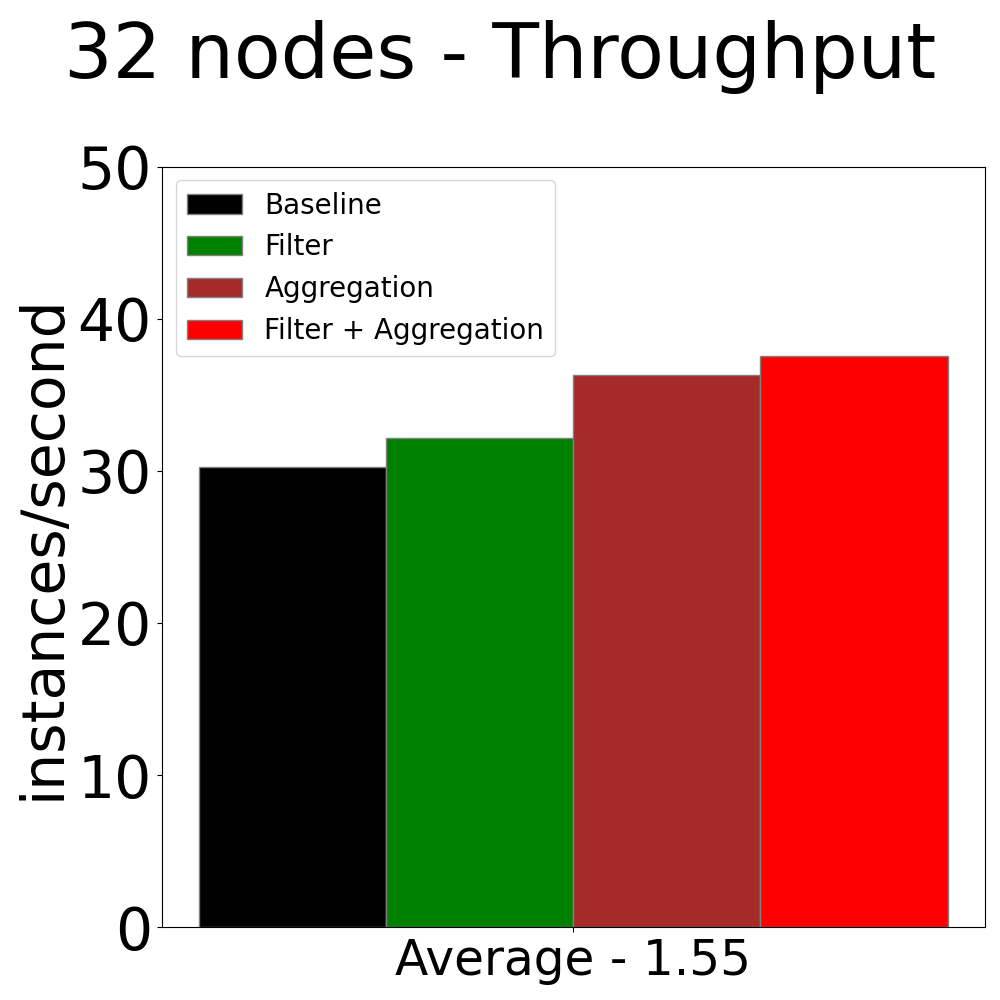
\includegraphics[%width=\columnwidth,
 height=4cm]{figures/thr-hist-32n.png}
	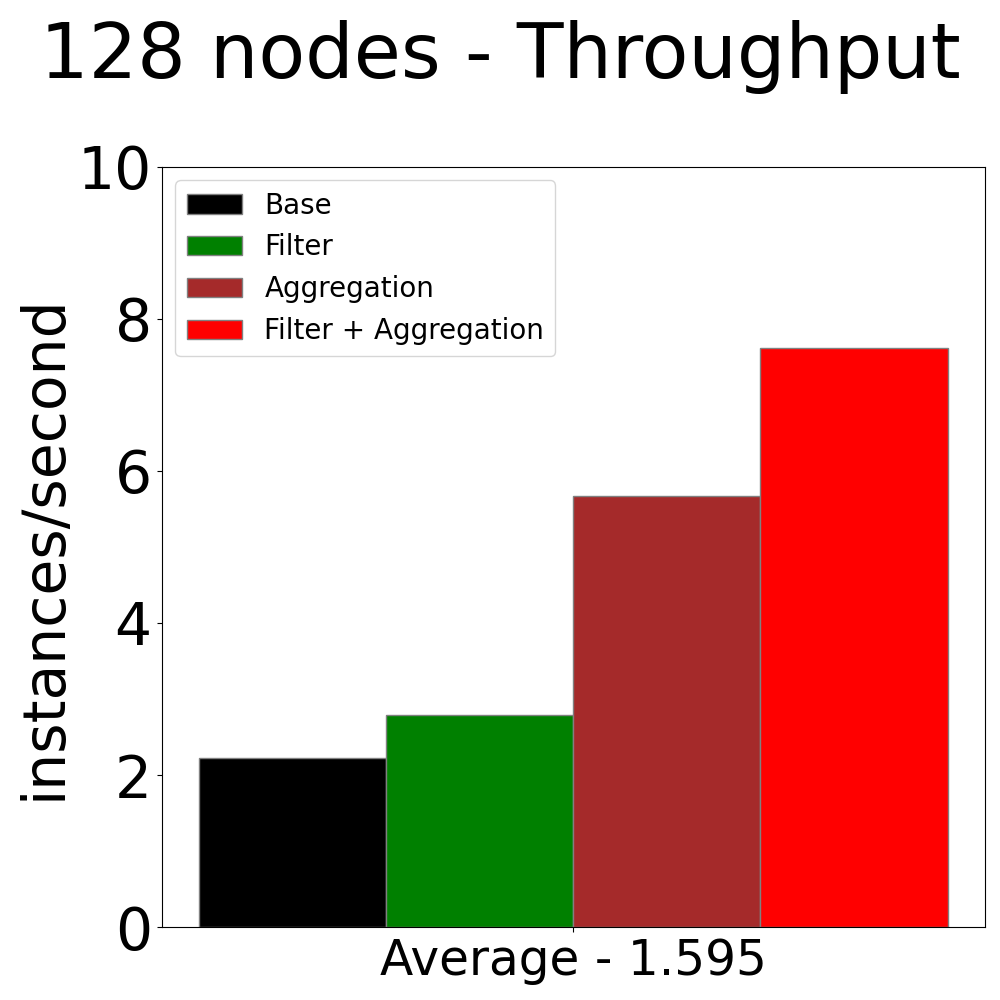
\includegraphics[%width=\columnwidth,
 height=4cm]{figures/thr-hist-128n.png}
	\caption{Comparison of throughput of the best throughput/latency relation points for Baseline, Filter, Aggregation and Filter+Aggregation for 32 (left) and 128 (right) nodes, for the average distance topology.}
	\label{fig:throughputComparisonAtSaturationPoint}
\end{figure}

Figure~\ref{fig:throughputComparisonAtSaturationPoint} shows the performance of Tendermint
in the four setups:  Baseline, Filtering, Aggregation, Filtering+Aggregation, for 32 nodes and 128 nodes.
Each bar represents the throughput at the sample with the best throughput/latency relation for each case.
This also is depicted with Table \ref{tab:sturationPoints}: for each Semantic Gossip setup,
the absolute and relative to the baseline numerical values ('relative' line) are shown.



%\begin{figure*}[htbp]
%\centering
%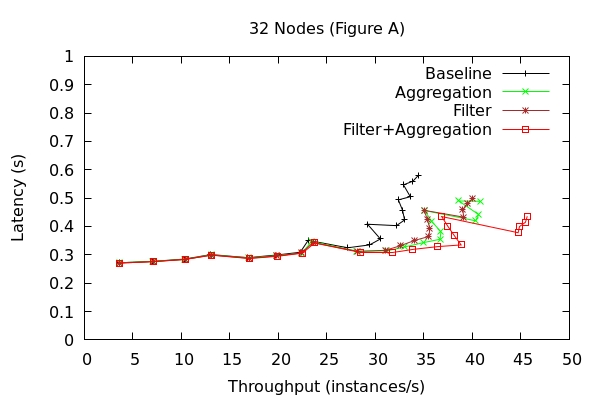
\includegraphics[width=\columnwidth]{figures/32nodes-avg-lat.png}
%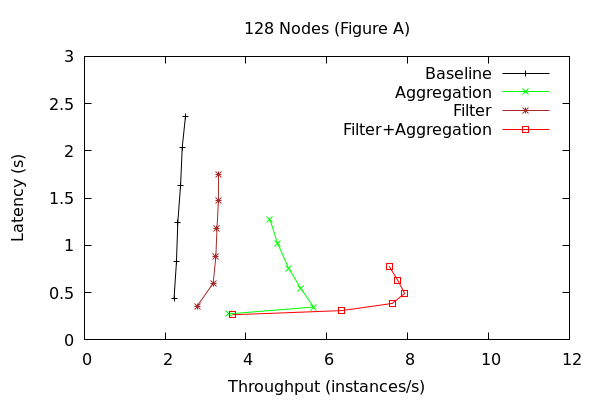
\includegraphics[width=\columnwidth]{figures/128nodes-avg-lat.png}
%\caption{Overall performance of Baseline, Filter, Aggregation and Filter+Aggregation for 32 and 128 nodes}
%\label{fig:overallTendermint}
%\end{figure*}
%
%\begin{figure*}[htbp]
%\centering
%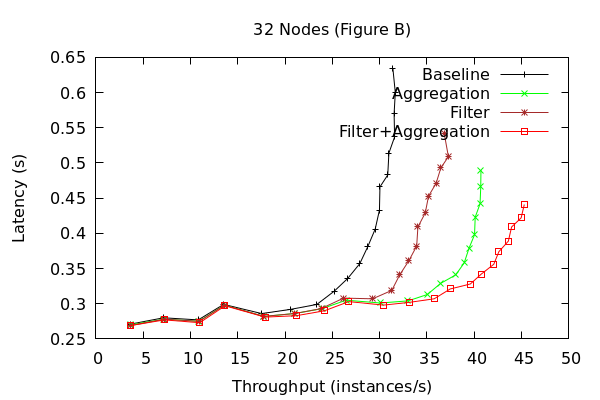
\includegraphics[width=\columnwidth]{figures/32nodes-eq-lats.png}
%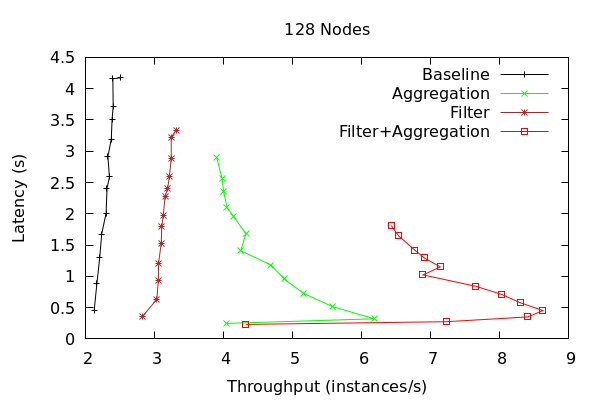
\includegraphics[width=\columnwidth]{figures/128nodes-eq-lats.png}
%\caption{Overall performance of Baseline, Filter, Aggregation and Filter+Aggregation for 32 and 128 nodes when all regions have equal latency between them}
%\label{fig:overallTendermintEqLats}
%\end{figure*}
%\rg{For 32 nodes it seems that using different latencies between regions have caused the issue of throughput decreasing and increasing "randomly", and the second plot shows something closer to our expectations. In the 128 nodes case the behaviour was essentially the same, but I ran the experiment with more points(more window sizes, up to 13). What I think is happening is that the aggregation is becoming less and less efficient as we increase the number of messages traveling on the network, because as we have more instances running concurrently we reduce the probability of a message be "close" in a receive buffer to other "aggregatable" messages. }
%
%\fd{For 32 nodes we experimented window varying from 1 to 20.  As can be seen, the throughput latency behavior has atypical variations.  In Fig 6, left, we show results for the same experiment, but adopting homogeneous latencies for all links in the topology.  As the window increases, different leaders are involved in ongoing instances. If a certain window size concentrates high latency leaders, its corresponding performance could be penalized.
%
% }

% \begin{figure}[htbp]
% \centering
% 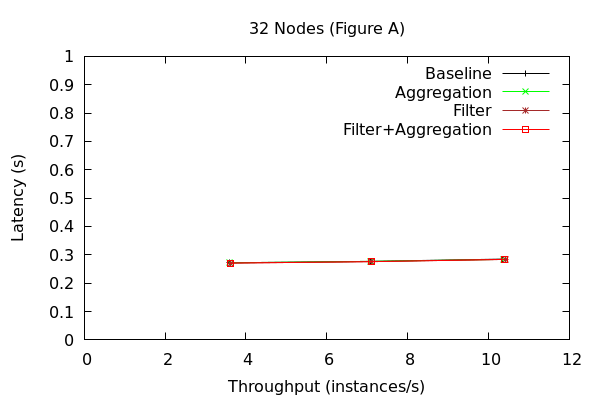
\includegraphics[width=\columnwidth]{figures/32nodes-3points.png}
% \caption{Close up of system performance with 32 nodes in the first three window sizes}
% \label{fig:cdfsW11}
% \end{figure}

%In the experiments with 32 nodes,
%the four setups perform almost equally until the Baseline reaches saturation (window  $\approx 10$, $\approx 30$ instances per second). 
With 32 nodes, the Baseline saturation point is reached with window 10, with several nodes showing average load\footnote{Linux measure meaning the number of processes which are either currently being executed by the CPU or are waiting for execution.} above the number of cores (8 in our experiment) revealing contention for CPU.  We also observed that  message handling is a main factor to CPU utilization.
%
As the mechanisms proposed spare messages, the demand for CPU is alleviated.   Thus, setups Filtering and Aggregation, in isolation, allow to further scale.  The combination of both, Filtering+Aggregation, leads to better performance than the isolated cases, reaching throughput 
1.24 $\times$ faster than the Baseline while slightly reducing latency.     

In experiments with 128 nodes the same is observed.  Due to the high number of nodes and consequent message handling demand, the Baseline setup shows saturation starting from window 1, again with average CPU load above the number of cores for several nodes.  Filtering and Aggregation alone again show positive results, shrinking latency and enhancing throughput.   Their combination allowed to reach 3.42 $\times$ the Baseline throughput showing latency compatible with 32 nodes on non-saturated setups.

\begin{table}[h!]
\centering
	\begin{tabular}{c c c c c }
	\hline
     Size in     &        &       &       & Filtering+  \\ 
	 Nodes & Baseline   & Filtering    & Aggregation    & Aggregation  \\  \hline
	32  		& 		30.261		&	32.145	&	36.271	&  37.559 \\
	relative   		& 		  1		&	1.06	&	1.20	&  1.24      \\ \hline
	128  		& 		2.223		&	2.791	&	5.672	&  7.618  \\  
	relative   		& 		  1		&	1.25	&	2.55	&  3.42  \\ \hline \\
 
	\end{tabular}
	\caption{Tendermint throughput for different network sizes and  gossip setups, at the best throughput/latency point.}
 \label{tab:sturationPoints}
 \vspace{-5mm}
\end{table}

\subsection{Mechanisms Working}

To better understand the effect of the mechanisms, we take the points with best throughput/latency relation and quantify their impact on message handling.   

Regarding Filtering, the results for setups Filtering and Filtering+Aggregation are depicted in Table \ref{tab:Filtering}.
With the 32 nodes network it shows that around 23\% of the messages were filtered out in both setups, while with 128 nodes around 30\% of the messages were filtered out.

\begin{table}[h!]
\centering
	\begin{tabular}{c c c c c }
	\hline
     Size in     &       &  Filtering+  \\ 
	 Nodes & Filtering    & Aggregation  \\  \hline
	32  		&	23.07\%	&  23.17\% \\
	128  		&	29.87\%	&  28.81\%  \\ \hline \\
	\end{tabular}
	\caption{Percentage of messages filtered out by the semantic filter mechanism at the best throughput/latency point.}
  \label{tab:Filtering}
\vspace{-3mm}
\end{table}

With Aggregation, we can observe in Table \ref{tab:Aggregation}
that the share of messages aggregated with others 
importantly increases with the number of nodes, revealing that indeed the phased and symmetric structure of the protocol lends itself for the usage of the Aggregation technique.

\begin{table}[h!]
\centering
	\begin{tabular}{c c c c c }
	\hline
     Size in     &       &  Filtering+  \\ 
	 Nodes & Aggregation    & Aggregation  \\  \hline
	32  		&	16.77\%	&  13.01\% \\
	128  		&	70.92\%	&  71.76\%  \\ \hline \\
	\end{tabular}
	\caption{Percentage of messages aggregated  at the best throughput/latency point.}
   \label{tab:Aggregation}
 \vspace{-5mm}
\end{table}
%\fd{just reminding.  this is the percentage of messages that were aggregated with others.  it does not measure exactly how many less messages were sent due aggregation.}

% \rg{One thing that maybe is interesting to mention here is that we have 23\% on the execution that were filtered out and we also have a difference of 24\% between the recvMsg/(numNodes*instances) ratios of the Baseline and the Filtering(19.25/25.14 at table III). In other words, as we skip sending 23\% of the messages, the nodes receive 24\% less messages per instance in comparison to the Baseline. Same way, we had 30\% of messages filtered out for 128 nodes and they received 33\% less messages per instance compared to the Baseline.}

% \fd{yes ... i am thinking that table II seems a fundamental measure  and maybe other measures just collapse to that...}


\subsection{Gossip messages per consensus instance}

To further evaluate the impact, we compute the average number of gossip messages received per node to complete a consensus instance. 

In an analytical approximation, for a network of $n$ nodes, each of which having $k$ neighbors, 
considering that a gossiped message reaches every node and each node forwards it once to its neighbors, we have that in average every node should receive $n * k/n = k$ copies of a gossiped message.
%
%Now, considering that we have one gossip diffusion for the $Propose$ step and $n$ gossips for the $Prevote$ and $Precommit$ steps, our estimation is that for every instance of consensus a node should receive $2nk$ gossiped messages. 
Now, considering that after the $Propose$ by the coordinator, each of the $n$ nodes gossips the $Prevote$ and then gossips the $Precommit$, our estimation is that for every instance of consensus a node should receive $2nk$ gossiped messages. 
For instance, with $n =32$ and $k = 13.87$, a consensus instance would lead each node to receive 
$\sim 887$ messages, while with $n =128$ and $k = 51.43$, would be $\sim 13.166$ messages.
However, as a node doesn't need every message to progress, and, depending on messages received, may skip phases, this upper bound should not be meet in practice.

In Table \ref{tab:msgsRcvdPerInstance} we depict the observed number of gossip messages handled per node, per consensus instance, for the several setups.   The baseline values are 7,9\% and 2,8\% under the estimated upper bound.
We notice that Filtering showed reduction  of 26\% and 31\% of messages respectively for 32 and 128 nodes. As discussed, 
Aggregation shows high impact as the number of nodes increase, here with 17\% and 75\% less messages for 32 and 128 nodes respectively.  Again, the mechanisms combined show still better effect than in isolation for both network sizes.

%\rg{Note that a network is built from a number $n$ of nodes, each of which has $k$ neighbors, each message is sent only once and every process should receive this message eventually. Thus every node should receive $n * k/n = k$ messages every time another node gossips a message. The number of gossip attempts per instance is $2n$, since we have one gossip diffusion for the $Propose$ step and $n$ gossips for the $Prevote$ and $Precommit$ steps. So our estimation says that for every instance of consensus a node should receive $2nk$ gossiped messages. But we should never meet this upper bound is practice, because a node doesn't needs every message to progress, only two thirds.}

%\rg{It seems that the filtering is more effective in smaller networks and aggregation in bigger ones. Another thing worth mentioning is that the aggregation is less and less effective as we increase the concurrency window size, as it is "opportunistic" in it's way of selecting the messages it should aggregate(it looks for the first 500 or something inside the "sendMessageBuffer"). }
%\fd{too much detail for this version}

\begin{table}[h!]
\center
	\begin{tabular}{c c c c c c }
	\hline
     Size in   & Estimated &   Base-    & Filte-      & Aggre-     & Filter.+  \\ 
	 Nodes & upper bound &     line   &   ring     &   gation    & Aggreg.  \\  \hline
	32  		& 887 & 		822,2        &	612,6	&	690,6	&  537,9 \\
 	relative   	& 1,079    & 		  1		     &	0,74	&	0,83	&  0,65      \\ \hline
	128  		& 13.166 & 		12.805,4   &	8.876,3	&	3.613,1	&  2471  \\ 
 	relative   	&  1,028   & 		  1		     &	0,69	&	0,25	&  0,19      \\ \hline \\
	\end{tabular}
	\caption{Average of gossip received messages per node, per decided Tendermint instance, at the best throughput/latency point.}
  \label{tab:msgsRcvdPerInstance}
 \vspace{-5mm}
\end{table}


\subsection{Latencies}
\label{sec:latency-cdfs}

Window 1 represents the situation where an instance of consensus is proposed only after the previous has been finished, therefore with minimum contention.
%
For 32 nodes and window 1, we observe in Figure \ref{fig:cdfs}(center) that all setups have the same latency distribution (lines are collapsed).  This means that the semantic mechanisms neither help nor impacted latency in this light scenario.

Interestingly, from Figure \ref{fig:cdfs} we observe that with 128 nodes, window 1 (right), the setups with Aggregation show latency distribution very similar to the reported with 32 nodes, window 1 (center), while the Filtering and Baseline show higher latency, in this order.
%
This emphasizes the 
importance of Aggregation as the number of nodes grows.  As Tendermint uses communication steps with the same types of messages addressed to all participants, the population of messages prone to Aggregation in intermediate nodes, and thus the positive impact of Aggregation, is proportional to the number of nodes.  
%

%leaving to conclude that Aggregation 
%this setup reduced communication overhead to be compatible with having $1/4$ of nodes.

%\fd{really?}   \rg{I think that saying it's "compatible with another size" it's a little bit problematic because the number of messages depends on K as well, and also the number of gossiped messages per instance of 128 nodes with filter+aggreg is three times the theoretical upper bound(2kn) we have for 32 nodes when k is 9. So, saying its "compatible with N" without specifying a K it's not very precise. What I think we can say is that we ...?  }

To detail the behavior with 32 nodes we take from the less performing setup (Baseline) the window with best throughput/latency point (window 13).
With this configuration all setups show similar throughput.
The latency distributions of the four setups is depicted in Figure \ref{fig:cdfs} (left).  %As the Baseline reaches saturation, 
Latency distributions are slightly better using Semantic Gossip. Aggregation shows  better impact than Filtering, and their combination further reduces latency.   

An important general observation is that the mechanisms are not delaying instance's decision, even if messages are dropped due to filtering.  On the contrary, latency distributions are consistently better at all percentiles with the mechanisms proposed, showing that sparing redundancy is indeed possible and a good measure.

\begin{figure*}[htbp]
\centering
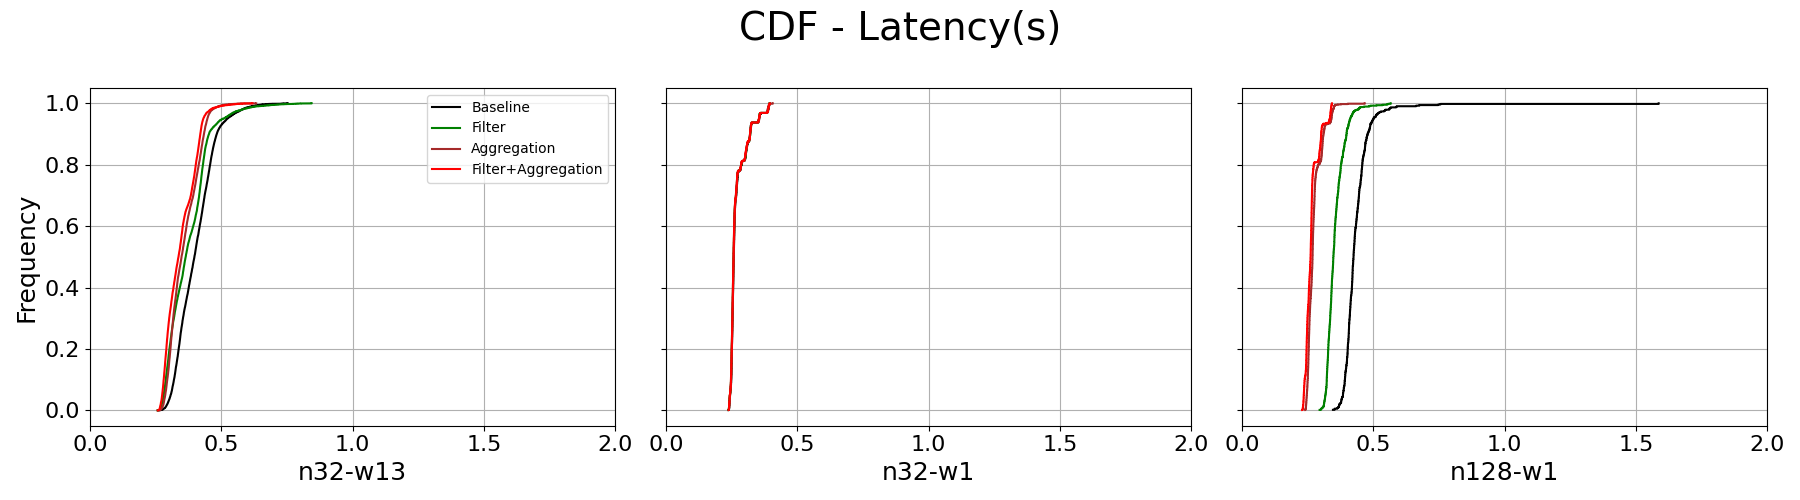
\includegraphics[width=\textwidth, height=4cm]{figures/cdfs.png}
\caption{Latency CDFs for Baseline, Filter, Aggregation and Filter+Aggregation, using window 13 for 32 nodes (left), window 1 for 32(center) and window 1 for 128 nodes(right)}
\label{fig:cdfs}
\end{figure*}


% \begin{figure*}[htbp]
% \centering
% 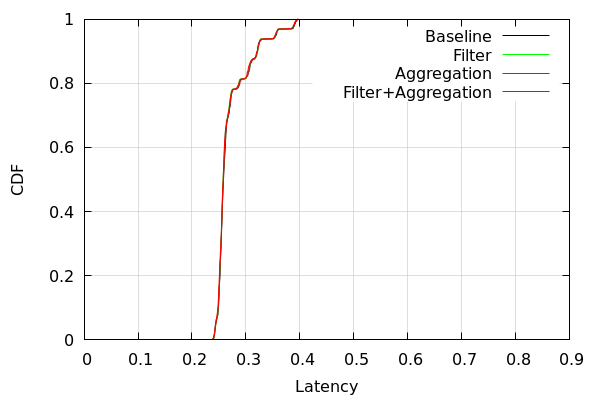
\includegraphics[width=\columnwidth]{figures/w1-32nodes-cdf.png}
% 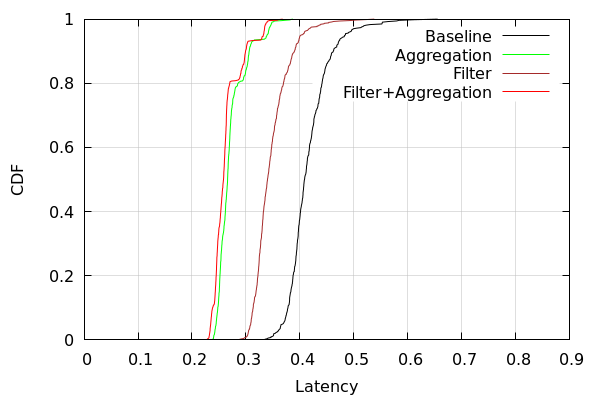
\includegraphics[width=\columnwidth]{figures/128nodes-cdf.png}
% 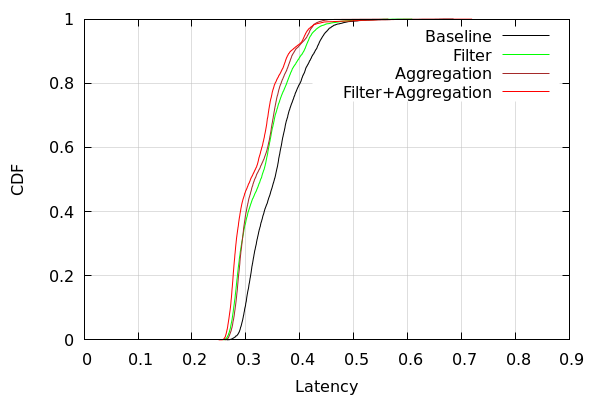
\includegraphics[width=\columnwidth]{figures/w11-32nodes-cdf.png}
% \caption{Latency CDFs for Baseline, Filter, Aggregation and Filter+Aggregation, using window 1 for 32 nodes (left) and  128 nodes(right)}
% \label{fig:cdfs}
% \end{figure*}

% \begin{figure}[htbp]
% \centering
% \caption{Latency CDf for 32 nodes Window size 11}
% \label{fig:cdfsW11}
% \end{figure}

\subsection{Resilience}
\label{sec:resilience}
\fd{SHOULD WE KEEP THIS OR DO THE MESSAGE LOSS STUDY?}

As redundancy is needed to cope with byzantine behavior and since Semantic Gossip is designed to safely eliminate redundancy, we designed experiments to evaluate if and how consensus is affected by byzantine behavior using Semantic Gossip mechanisms in comparison to the Baseline.

Under the assumption that signatures are reliable and since gossip works with signature verification, any attempt to forge or corrupt messages would be detected.   Therefore, we conclude the worst byzantine behavior to harm consensus would be that dishonest nodes remain silent, i.e. they do not collaborate with the consensus protocol.

For 32 and 128 nodes, we incrementally convert honest to byzantine nodes, 5 by 5\%, starting with 0 and going up to 30\%.  Regardless of performance, consensus should show progress in all cases since it supports up to $1/3$ dishonest nodes.  Tables \ref{tab:biz32} and \ref{tab:biz128} show the resulting throughput of the experiment respectively for 32 and 128 nodes.  The first general observation is that all configurations keep progress.   The second is that for 128 nodes all Semantic Gossip configurations performed better than or equivalent to the Baseline.  Thirdly, for 32 nodes, in all configurations the effect of having Filtering+Aggregation slightly enhanced or has equivalent throughput.   For Filtering and Aggregation separated, in most cases performance was equivalent or better than the Baseline.  For 30\% dishonest nodes these setups show performance below the Baseline, indicating that message drop by the mechanisms, added by 30\% of silent nodes, have slightly delayed consensus to be reached.

\begin{table}[h!]
\centering
	\begin{tabular}{c c c c c }
	\hline
     Byzantine     &        &       &       & Filtering+  \\ 
	 Nodes & Baseline   & Filtering    & Aggregation    & Aggregation  \\  \hline
	 0 \%  		    & 		1		&	1	&	1	& 1  \\
	 5 \%  		    & 		0.044		&	0.041	&	0.040	& 0.037  \\
	 10 \%  		& 		0.022		&	0.020	&	0.021	& 0.019  \\
	 15 \%  		& 		0.022		&	0.020	&	0.020	& 0.018  \\
	 20 \%  		& 		0.021		&	0.017	&	0.019	& 0.018  \\
	 25 \%  		& 		0.017		&	0.019	&	0.023	& 0.023  \\
	 30 \%  		& 		0.017		&	0.010	&	0.009	& 0.016  \\ \hline \\
	\end{tabular}
	\caption{Tendermint throughput in instances/sec with 32 nodes. 
 Each setup with window of best throughput/latency point with 0 dishonest nodes.   Then converting nodes 5 by 5\% to dishonest.}
 \label{tab:biz32}
\end{table}

\begin{table}[h!]
\centering
	\begin{tabular}{c c c c c }
	\hline
     Byzantine     &        &       &       & Filtering+  \\ 
	 Nodes & Baseline   & Filtering    & Aggregation    & Aggregation  \\  \hline
	 0 \%  		    & 		1		&	1	&	1	& 1  \\
	 5 \%  		    & 		0.329		&	0.249	&	0.173	& 0.131  \\
	 10 \%  		& 		0.200		&	0.153	&	0.094	& 0.065  \\
	 15 \%  		& 		0.157		&	0.115	&	0.075	& 0.051  \\
	 20 \%  		& 		0.116		&	0.085	&	0.051	& 0.035  \\
	 25 \%  		& 		0.100		&	0.073	&	0.042	& 0.039  \\
	 30 \%  		& 		0.083		&	0.068	&	0.062	& 0.052  \\ \hline \\
	\end{tabular}
	\caption{Tendermint throughput in instances/sec with 128 nodes. 
 Each setup with window of best throughput/latency point with 0 dishonest nodes.   Then converting nodes 5 by 5\% to dishonest.}
  \label{tab:biz128}
\end{table}



% \fd{a análise acima é válida.   acho que podemos seguir pela vazao.
% adicionando grafico de thoughput/latencia podemos mostrar que os mecanismos nao prejudicam latencia}


% talvez possamos usar latencia ...

% PARA RESPONDER QUE OS MECANISMOS NAO IMPEDEM A DECISAO,  PODEMOS PEGAR O CASO DE JANELA 1 E VER A LATENCIA PARA DECISOES.   SE A LATENCIA PARA DECISAO FOR MAIOR QUE PARA O BASELINE, EM TESE ALGUMA MENSAGEM ESTA SENDO JOGADA FORA E NAO DEVERIA.   SE TIVER LATENCIA MELHOR, AINDA MELHOR.

% UM ESTUDO ADICIONAL SERIA SUPONDO O SISTEMA EM ALTA UTILIZCAO, COMO IMPACTAM OS BIZANTINOS EM CADA CASO.
% AQUI PEGARIA O CENARIO DE MELHOR THROUGHPUT/LATENCIA EM CADA CASO.
% DAI TERIA QUE PLOTAR O GRAFICO THROUGHPUT/LATENCIA,
% E UMA TABELA DE LATENCIA MEDIA POR INSTANCIA. 


\subsection{Message loss}
\label{sec:msgLoss}
In addition to Byzantine behaviors, a consistent consensus mechanism must also be tolerant of imperfect links that allow message loss. We implemented this feature by dropping messages, when they are received, with a predefined probability, so they are not computed by the consensus neither forwarded to other peers.   We measure latency and throughput of the different techniques with loss probabilities increasing 5 by 5 from 0 to 60\%, in a network of 32 nodes.   With window 1,   we observe a gradual degradation of the performance, both for throughput and latency, until we arrive at 50 to 60\% message loss.   With window 13,  
%
%This way, we are able to measure the impacts of faulty links on Tendermint's performance, with and without the Semantic Gossip techniques. 
%
%Now, since the Semantic Filtering reduces the total amount of messages per consensus instances to the minimum needed for termination and Semantic Aggregation may lead to several messages being dropped at once, we also evaluate whether these techniques make the system more susceptible to postponement due to message loss.
%
%We incremented the message loss probability 5 by 5\%, starting from 0, but going up to 60\%. We evaluated this scenario exclusively for the 32 nodes configuration because...(should we argue something here?). 
Figures \ref{fig:msgLossThroughput} and \ref{fig:msgLossLatency} show that we have a gradual degradation of the performance,  until we arrive at 30\% message loss, where the number of decided instances drops abruptly. The baseline has this threshold point with 35\% message loss. 
%
%This behavior is spread among all the experimented setups, which leads us to the conclusion that no vulnerability was introduced by our Semantic Gossip module regarding message loss tolerance. 
%
This shows that, with Semantic Gossip filtering and aggregation, the system operates with performance better than the Baseline even under loss rates up to 30\%.


%the degree of redundancy of the gossip propagation method is very high, allowing the system to operate with performance similar to the case without failures with up to 30\% message loss.\fd{revise this ...}


%\begin{figure}[htbp]
%	\centering
%	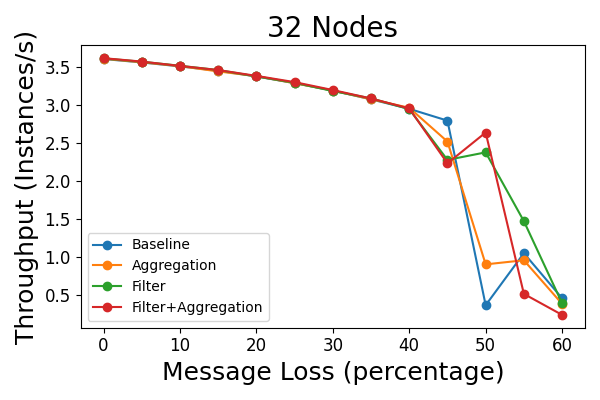
\includegraphics[%width=\columnwidth,  height=5cm]{figures/msgloss-diff-lat-32nodes-loss-thr.png}
	
%\caption{Tendermint throughput in instances/s with 32 nodes. Setups with window size equals one. Message loss percentage incremented 5 by 5.}
	%\label{fig:msgLossThroughput}
%\end{figure}

%\begin{figure}[htbp]
%	\centering  
	%\includegraphics[%width=\columnwidth, height=5cm]{figures/msgloss-diff-lat-532nodes-loss-lat.png}
%	\caption{Tendermint latency in seconds with 32 nodes. Setups with window size equals one. Message loss percentage incremented 5 by 5.}
	%\label{fig:msgLossLatency}
%\end{figure}



\begin{figure}[htbp]
	\centering
	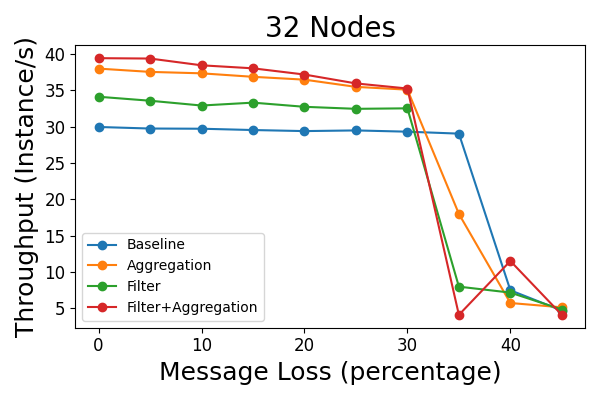
\includegraphics[%width=\columnwidth,
  height=5cm]{figures/w13-msgloss-32nodes-loss-thr.png}
	\caption{Tendermint throughput in instances/s with 32 nodes. Setups with window size equals 13. Message loss percentage incremented 5 by 5.}
	\label{fig:msgLossThroughput}
\end{figure}

\begin{figure}[htbp]
	\centering  
	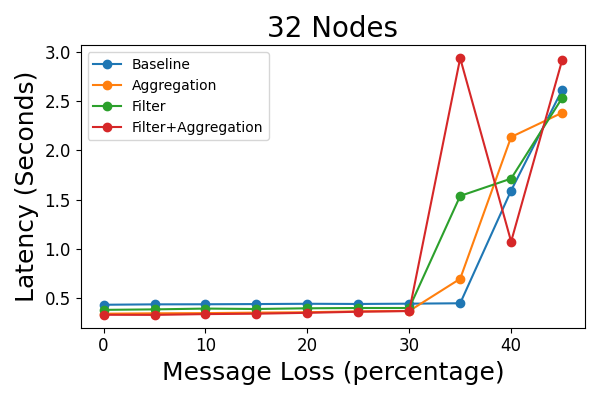
\includegraphics[%width=\columnwidth, 
     height=5cm]{figures/w13-msgloss-32nodes-loss-lat.png}
	\caption{Tendermint latency in seconds with 32 nodes. Setups with window size equals 13. Message loss percentage incremented 5 by 5.}
	\label{fig:msgLossLatency}
\end{figure}

\label{sec:signatureImpact}


% \begin{table}[h!]
% 	\begin{tabular}{c c c c c }
% 	\hline
%      Signature     &        &       &       & Filtering+  \\ 
% 	 Validation & Baseline   & Filtering    & Aggregation    & Aggregation  \\  \hline
% 	  on  		& 		...		&		&		&   \\
% 	  off  		& 				&		&		&    \\ \hline \\
% 	\end{tabular}
% 	\caption{Saturation point throughput using signature validation, or not, with 
% 	none (Baseline), Filtering,
% 	Aggregation and Filtering and Aggregation semantic gossip mechanisms with Tendermint.}
% \end{table}

% \rg{We have to discuss better the data. }


